\documentclass[aspectratio=169,11pt]{beamer}
\usepackage[T1]{fontenc}
\usepackage{lmodern,microtype}
\usepackage{amsmath,amssymb,mathtools}
\usepackage{tikz}
\usetikzlibrary{arrows.meta,positioning,calc}
\definecolor{cream}{HTML}{F7F5EE}
\definecolor{navy}{HTML}{193247}
\definecolor{teal}{HTML}{137D89}
\definecolor{muted}{HTML}{657783}
\definecolor{pale}{HTML}{DCECE9}
\definecolor{rust}{HTML}{B9623C}
\definecolor{grid}{HTML}{C5D0D1}
\setbeamercolor{background canvas}{bg=cream}
\setbeamercolor{normal text}{fg=navy,bg=cream}
\setbeamercolor{frametitle}{fg=navy,bg=cream}
\setbeamercolor{structure}{fg=teal}
\setbeamercolor{alerted text}{fg=teal}
\setbeamercolor{item}{fg=teal}
\setbeamertemplate{navigation symbols}{}
\setbeamertemplate{itemize item}{\small\raisebox{0.1ex}{$\bullet$}}
\setbeamersize{text margin left=9mm,text margin right=9mm}
\setbeamerfont{frametitle}{size=\fontsize{21}{24},series=\bfseries}
\setbeamerfont{title}{size=\Huge,series=\bfseries}
\setbeamertemplate{frametitle}{\vspace{3mm}\insertframetitle\par\vspace{2mm}{\color{teal}\rule{\textwidth}{0.65pt}}}
\newcommand{\slidesource}{}
\newcommand{\source}[1]{\gdef\slidesource{#1}}
\setbeamertemplate{footline}{%
\begin{beamercolorbox}[wd=\paperwidth,ht=8mm,dp=2mm,leftskip=9mm,rightskip=9mm]{normal text}%
\hbox to\dimexpr\paperwidth-18mm\relax{%
\parbox[b]{132mm}{\fontsize{6.4}{7.8}\selectfont\color{muted}\slidesource}%
\hfil{\fontsize{8}{9}\selectfont\color{muted}\insertframenumber}}%
\end{beamercolorbox}}
\newcommand{\E}{\mathbb E}
\newcommand{\PP}{\mathbb P}
\newcommand{\1}{\mathbf 1}
\newcommand{\Pcal}{\mathcal P}
\newcommand{\takeaway}[1]{\par\vspace{2mm}{\color{teal}\bfseries #1}\par}
\newcommand{\smallgap}{\vspace{2mm}}
\newcommand{\cellgrid}{\draw[grid,step=0.45] (0,0) grid (2.25,2.25);}
\hypersetup{pdftitle={Problem 21: Why centering helps a random matching},pdfauthor={},pdfsubject={A direct proof of the centered permutation product estimate and its spectral application},colorlinks=true,urlcolor=teal}
\title{Why centering helps\protect\\a random matching}
\author{}
\date{Problem 21\quad November 2026}
\pdfinfoomitdate=1
\pdftrailerid{}
\pdfsuppressptexinfo=15
\begin{document}
\setlength{\abovedisplayskip}{7pt}
\setlength{\belowdisplayskip}{7pt}
\setlength{\abovedisplayshortskip}{4pt}
\setlength{\belowdisplayshortskip}{4pt}

\source{Problem 21 submission. The report contains the full proofs, source audit and tool-use record.}
\begin{frame}[plain]
\vspace{5mm}
{\color{teal}\normalsize PROBLEM 21}\par\vspace{5mm}
\begin{columns}[T,onlytextwidth]
\begin{column}{0.69\textwidth}
{\fontsize{26}{30}\selectfont\bfseries Why centering helps\\a random matching}\par
\vspace{5mm}
{\large A direct proof of Proposition 28}\par
\smallgap
{\large and its biregular spectral-gap input}\par
\vspace{7mm}
{\color{muted}\normalsize Keep cancellation. Condition exactly. Sum a row.}
\par\vspace{3mm}
{\color{muted}\normalsize\insertauthor}
\end{column}
\begin{column}{0.27\textwidth}
\centering
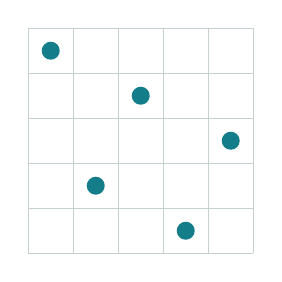
\begin{tikzpicture}[scale=1.27]
\cellgrid
\foreach \x/\y in {0.225/2.025,0.675/0.675,1.125/1.575,1.575/0.225,2.025/1.125}{\fill[teal] (\x,\y) circle (0.09);}
\end{tikzpicture}
\end{column}
\end{columns}
\vfill
{\color{navy}\large From one matching product to the non-backtracking argument}
\end{frame}

\source{Report: ``The question and the proof mechanism'', two-cell calculation.}
\begin{frame}{Two cells reveal cancellation}
\begin{columns}[T,onlytextwidth]
\begin{column}{0.48\textwidth}
\centering
{\bfseries Different rows and columns}\par\smallgap
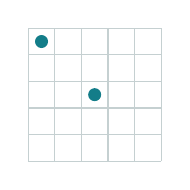
\begin{tikzpicture}[scale=0.75]
\cellgrid
\fill[teal] (0.225,2.025) circle (0.11);
\fill[teal] (1.125,1.125) circle (0.11);
\end{tikzpicture}
\[
\E[(M_{11}-N^{-1})(M_{22}-N^{-1})]
\]
\vspace{-3mm}
\[
=\frac1{N(N-1)}-\frac1{N^2}
=\alert{\frac1{N^2(N-1)}}.
\]
\end{column}
\begin{column}{0.48\textwidth}
\centering
{\bfseries Two cells in one row}\par\smallgap
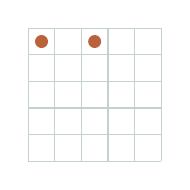
\begin{tikzpicture}[scale=0.75]
\cellgrid
\fill[rust] (0.225,2.025) circle (0.11);
\fill[rust] (1.125,2.025) circle (0.11);
\end{tikzpicture}
\[
\E[(M_{11}-N^{-1})(M_{12}-N^{-1})]
\]
\vspace{-3mm}
\[
=\alert{-\frac1{N^2}}.
\]
\end{column}
\end{columns}
\smallgap
\centering\small Dots are requested cells, not a realized permutation.
\takeaway{The pattern matters. Absolute values taken too early lose the gain.}
\end{frame}

\source{Report: ``An attained envelope for mixed products'', definition of the mixed product and consistency.}
\begin{frame}{Which centered factors earn a gain?}
Each color $c$ has an independent uniform permutation of $[N]$, with $N\ge2$.
\[
M_{cij}=\1_{\{\sigma_c(i)=j\}},\qquad
P=\prod_{e\in E}(M_e-N^{-1})^{p_e}M_e^{q_e}.
\]
\vspace{1mm}
\begin{tabular}{@{}p{0.12\textwidth}p{0.83\textwidth}@{}}
\alert{$a=|E|$} & Number of distinct requested cells. Multiplicities are arbitrary.\\[3mm]
\alert{$h$} & Consistent centered singletons: $(p_e,q_e)=(1,0)$, with no other requested cell of that color in their row or column.\\[3mm]
\alert{$b$} & The other centered singletons, which share a row or column with a requested cell of the same color.
\end{tabular}
\takeaway{Consistency is a property of the requested pattern before sampling.}
\end{frame}

\source{Report: Corollary ``Scalar mixed bounds''. Bordenave, Proposition 28, is recovered on slide 10.}
\begin{frame}{The product estimate}
For $2\le a\le\sqrt N$, with the counts $a,h,b$ just defined,
\vspace{3mm}
\[
\boxed{\displaystyle
|\E P|\le\sqrt e\,2^bN^{-a}
\left(\frac{\sqrt{a-1}}{\sqrt N-\sqrt{a-1}}\right)^h.}
\]
\vspace{4mm}
\begin{columns}[T,onlytextwidth]
\begin{column}{0.29\textwidth}
\centering\alert{\Large $N^{-a}$}\par\smallgap
One matching cost for each distinct cell
\end{column}
\begin{column}{0.29\textwidth}
\centering\alert{\Large $2^b$}\par\smallgap
A cost for conflicting centered singletons
\end{column}
\begin{column}{0.34\textwidth}
\centering\alert{\Large $\bigl(O(\sqrt{a/N})\bigr)^h$}\par\smallgap
An extra gain for each consistent singleton
\end{column}
\end{columns}
\takeaway{Preserve the $h$ centered singletons while handling every other factor.}
\end{frame}

\source{Report: ``Exact depleted moments''. Only a compatible prescribed set is exposed.}
\begin{frame}{Condition on compatible matches}
Prescribe $r$ matches with distinct rows and columns.
\[
\PP(\text{all prescribed matches occur})=\frac1{(N)_r}.
\]
\vspace{-1mm}
\begin{columns}[c,onlytextwidth]
\begin{column}{0.46\textwidth}
\centering
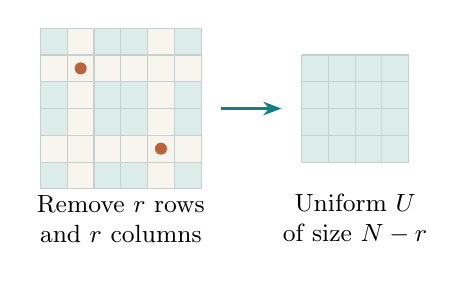
\begin{tikzpicture}[scale=0.85]
\fill[pale] (0,0) rectangle (2.4,2.4);
\fill[cream] (0,1.6) rectangle (2.4,2.0);
\fill[cream] (0,0.4) rectangle (2.4,0.8);
\fill[cream] (0.4,0) rectangle (0.8,2.4);
\fill[cream] (1.6,0) rectangle (2.0,2.4);
\draw[grid,step=0.4] (0,0) grid (2.4,2.4);
\fill[rust] (0.6,1.8) circle (0.09);
\fill[rust] (1.8,0.6) circle (0.09);
\draw[-{Stealth},thick,teal] (2.7,1.2) -- (3.6,1.2);
\begin{scope}[shift={(3.9,0.4)}]
\fill[pale] (0,0) rectangle (1.6,1.6);
\draw[grid,step=0.4] (0,0) grid (1.6,1.6);
\end{scope}
\node[font=\small,align=center] at (1.2,-0.45) {Remove $r$ rows\\and $r$ columns};
\node[font=\small,align=center] at (4.7,-0.45) {Uniform $U$\\of size $N-r$};
\end{tikzpicture}
\end{column}
\begin{column}{0.49\textwidth}
Keep the original centering $1/N$:
\[
Z_{ij}=NU_{ij}-1.
\]
Since each row of $U$ sums to one,
\[
\alert{\sum_v Z_{iv}=N-(N-r)=r.}
\]
\end{column}
\end{columns}
\takeaway{The remaining row sum is $r$, not zero.}
\end{frame}

\source{Report: Lemma ``Depleted row-sum recurrence''. At r = 0, the rescaled recurrence is Collins and Nagatsu, Proposition 3.3.}
\begin{frame}{A row sum gives the recurrence}
Let $\mu_j=\E\prod_{i=1}^j Z_{ii}$, with $\mu_0=1$ and $j+r\le N$.
\[
r\mu_{j-1}=\sum_v\E\!\left[Z_{jv}\prod_{i<j}Z_{ii}\right].
\]
\vspace{-2mm}
\begin{columns}[T,onlytextwidth]
\begin{column}{0.45\textwidth}
\alert{Unused column}\par\smallgap
$N-r-j+1$ choices, each with moment $\mu_j$.
\end{column}
\begin{column}{0.51\textwidth}
\alert{Used column $i<j$}\par\smallgap
The indicators conflict, so
\[
Z_{ii}Z_{ji}=-Z_{ii}-Z_{ji}-1.
\]
\end{column}
\end{columns}
\vspace{1mm}
\[
\boxed{(N-r-j+1)\mu_j
=(r+2j-2)\mu_{j-1}+(j-1)\mu_{j-2}.}
\]
\centering\small Omit the last term at $j=1$. All coefficients on the right are nonnegative.
\end{frame}

\source{Report: Lemma ``A geometric supersolution'', using its simpler beta bound.}
\begin{frame}{Positivity gives a scalar bound}
Start with $\mu_0=1$ and $\mu_1=r/(N-r)$. Then $\mu_j\ge0$.
For $r+h\le a$ and $2\le j\le h$, the recurrence is bounded by
\[
\mu_j\le
\frac{2(a-1)\mu_{j-1}+(a-1)\mu_{j-2}}{N-a+1}.
\]
\smallgap
Choose the positive root $\beta$ of
\[
(N-a+1)\beta^2=2(a-1)\beta+(a-1).
\]
\[
\beta=\frac{\sqrt{a-1}}{\sqrt N-\sqrt{a-1}}
\qquad\Longrightarrow\qquad
\boxed{0\le\mu_h\le\beta^h.}
\]
\takeaway{The triangle inequality is safe after the positive recurrence is obtained.}
\end{frame}

\source{Report: proof of Theorem ``An attained mixed-product envelope'', affine coefficient weights.}
\begin{frame}{Repeated factors become affine}
Set the $h$ consistent centered singletons aside in a set $T$.
\smallgap
For every $e\notin T$, the identity $M_e^2=M_e$ gives
\[
(M_e-N^{-1})^{p_e}M_e^{q_e}=c_e+d_eM_e,
\qquad d_e\ge0.
\]
\vspace{2mm}
Its expansion has a controlled coefficient weight:
\[
d_e+N|c_e|\le
\begin{cases}
2,&(p_e,q_e)=(1,0),\\[1mm]
1,&\text{otherwise}.
\end{cases}
\]
\smallgap
Selecting an $M_e$ term prescribes a match. Incompatible selections vanish.
\takeaway{Repeated powers cost no extra factor. Only the $b$ remaining singletons cost two.}
\end{frame}

\source{Report: Lemma ``Monotonicity and merging'' and Corollary ``Scalar mixed bounds''.}
\begin{frame}{Merge colors and sum the terms}
Write $F_N(r)=N^r/(N)_r$ and $K_{j,r}=F_N(r)\mu_j(N,r)$.
The positive partition formula gives
\[
K_{j_1,r_1}K_{j_2,r_2}\le K_{j_1+j_2,r_1+r_2},
\qquad K_{j,r}\ \text{increases with }r.
\]
For a compatible selected set $S$, conditioning gives exactly
\[
\E\!\left[\prod_{e\in S}M_e\prod_{e\in T}(M_e-N^{-1})\right]
=N^{-h-|S|}\prod_cK_{h_c,r_c}\ge0.
\]
After merging and summing coefficient weights,
\[
|\E P|\le 2^bN^{-a}F_N(a-h)\mu_h(N,a-h)
\le\alert{\sqrt e\,2^bN^{-a}\beta^h}.
\]
\centering\small Here $a\le\sqrt N$ gives $\log F_N(a-h)\le\tfrac12$.
\end{frame}

\source{Bordenave (2020), Proposition 28. Report: ``Random lifts: one permutation per base edge''.}
\begin{frame}{Recovering Proposition 28}
In a random lift, each chosen base-edge orientation carries one permutation.
\begin{itemize}
\setlength{\itemsep}{2mm}
\item Base edges are colors. Reverse traversal uses the same permutation transposed.
\item Distinct requested lift edges are cells.
\item Bordenave's $a_1$ is the count $h$ of consistent centered singletons.
\end{itemize}
\vspace{2mm}
For $k$ factors, $a\le k\le\sqrt N$, and $a\ge2$,
\[
|\E P|\le\sqrt e\,2^bN^{-a}
\underbrace{\bigl(2\sqrt{a/N}\bigr)^h}_{\text{our scalar consequence}}
\le\sqrt e\,2^bN^{-a}
\underbrace{\bigl(3k/\sqrt N\bigr)^{a_1}}_{\text{Proposition 28 form}}.
\]
\takeaway{The direct proof retains a stronger consistent-singleton factor.}
\end{frame}

\source{Brito, Dumitriu and Harris (2022), published Lemma 5.6, preprint Lemma 7. Report: biregular matching subsection.}
\begin{frame}{Biregular matching uses half-edges}
\begin{columns}[c,onlytextwidth]
\begin{column}{0.42\textwidth}
\centering
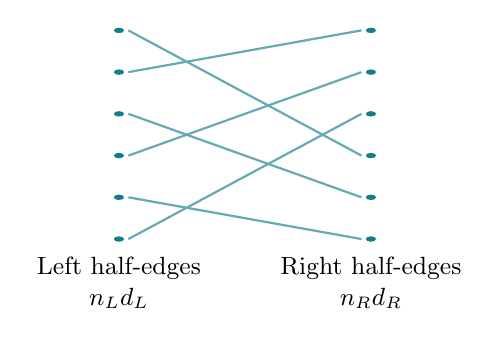
\begin{tikzpicture}[x=1cm,y=0.53cm]
\foreach \y in {0,1,2,3,4,5}{\fill[teal] (0,\y) circle (0.065);\fill[teal] (3.2,\y) circle (0.065);}
\foreach \a/\b in {0/3,1/0,2/4,3/1,4/5,5/2}{\draw[teal!65,thick] (0.12,\a) -- (3.08,\b);}
\node[align=center,font=\small] at (0,-1.05) {Left half-edges\\$n_Ld_L$};
\node[align=center,font=\small] at (3.2,-1.05) {Right half-edges\\$n_Rd_R$};
\end{tikzpicture}
\end{column}
\begin{column}{0.54\textwidth}
Both half-edge sets have size
\[
\alert{L=n_Ld_L=n_Rd_R.}
\]
Their uniform matching has matrix
\[
\begin{pmatrix}0&U\\U^{\mathsf T}&0\end{pmatrix},
\quad U\in\{0,1\}^{L\times L}.
\]
Apply the product theorem to $U$ with $N=L$.
\end{column}
\end{columns}
\takeaway{Center the random block at $1/L$. Same-side matching entries vanish.}
\end{frame}

\source{Report: ``Where the estimate enters spectral-gap arguments''. Graph enumeration and tangle estimates are separate inputs.}
\begin{frame}{The bridge to the adjacency spectrum}
\centering
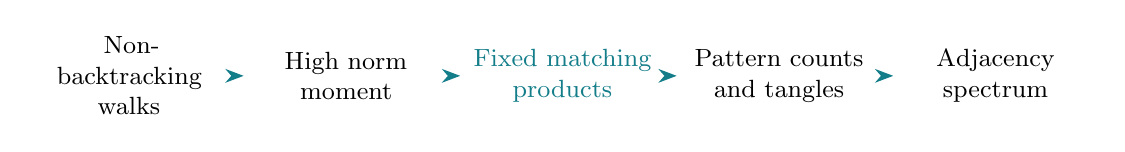
\begin{tikzpicture}[>=Stealth,every node/.style={align=center,font=\small,text width=2.35cm}]
\node (walk) at (0,0) {Non-backtracking\\walks};
\node (moment) at (2.75,0) {High norm\\moment};
\node[text=teal] (prod) at (5.5,0) {Fixed matching\\products};
\node (count) at (8.25,0) {Pattern counts\\and tangles};
\node (adj) at (11,0) {Adjacency\\spectrum};
\draw[->,teal,thick] (walk) -- (moment);
\draw[->,teal,thick] (moment) -- (prod);
\draw[->,teal,thick] (prod) -- (count);
\draw[->,teal,thick] (count) -- (adj);
\end{tikzpicture}
\vspace{0mm}
\raggedright
For a centered path matrix $C$, a norm bound valid without normality is
\[
\|C\|^{2s}\le\operatorname{tr}\bigl((CC^*)^s\bigr).
\]
Set $\alpha=d_L-1$ and $\gamma=d_R-1$, with $d_L,d_R\ge2$.
For a positive singular value $s_X$, the relation of Ihara and Bass is
\[
(z^2+\alpha)(z^2+\gamma)=s_X^2z^2.
\]
\centering\small
$s_X>\sqrt\alpha+\sqrt\gamma$ forces a root with $|z|>(\alpha\gamma)^{1/4}$.
\takeaway{We prove the matching-product input, not a new graph eigenvalue theorem.}
\end{frame}

\source{Report: Theorem ``An attained mixed-product envelope''. The one- and two-conflict theorems give further exact maxima.}
\begin{frame}{An exact maximum without conflicts}
For $1\le a\le N$, $0\le h\le a$ and $b=0$, the largest $|\E P|$ is
\[
\boxed{\displaystyle
\frac{N^{-h}\Pcal_h(N,a-h)}{(N)_a}.}
\]
The positive polynomial is $\Pcal_h(N,r)=(N-r)_h\mu_h(N,r)$.
Use one permutation and $a$ distinct diagonal cells to attain the bound:
\[
\prod_{i=1}^{h}(M_{ii}-N^{-1})
\quad\prod_{i=h+1}^{a}M_{ii}.
\]
\centering\small Center the first $h$ cells and take the remaining $a-h$ factors raw.
\takeaway{The report also treats one or two conflicting singletons and diagonal asymptotics.}
\end{frame}

\source{Tool-use disclosure. See the report for the expanded account.}
\begin{frame}{Tool use and verification scope}
\begin{tabular}{@{}p{0.26\textwidth}p{0.69\textwidth}@{}}
\textbf{OpenAI Codex} & Drafting, coding, proof exploration and internal review.\\[5mm]
\textbf{Python} & Exact finite checks of the recurrence, normalization and conditioning examples.\\[5mm]
\textbf{LaTeX} & Preparation of the report and slides, followed by visual inspection.\\[5mm]
\textbf{Limits} & Internal review and finite checks do not constitute an end-to-end formal proof or an audit of the full graph arguments.
\end{tabular}
\vspace{4mm}
\takeaway{The stated general inequalities rest on the symbolic proofs in the report.}
\end{frame}

\source{Bordenave (2020), equation (62), printed page 1428. Report: ``Two checks on a conditioning formula''.}
\begin{frame}{Backup: two exposed arrows}
For $N=4$, request $(1,1)$ and $(2,2)$, and condition on
\[
\sigma(2)=3,\qquad \sigma^{-1}(2)=4.
\]
This reveals two matches, $2\mapsto3$ and $4\mapsto2$.
\begin{columns}[c,onlytextwidth]
\begin{column}{0.51\textwidth}
\[
\text{Remaining rows: }\{1,3\},
\]
\vspace{-4mm}
\[
\text{remaining columns: }\{1,4\}.
\]
\end{column}
\begin{column}{0.45\textwidth}
\[
\alert{\PP(M_{11}=1\mid\text{exposure})=\frac12.}
\]
\end{column}
\end{columns}
The displayed source formula counts only one removed image and gives $1/3$.
\takeaway{This refutes the intermediate conditional assertion, not Proposition 28.}
\end{frame}

\source{Bibliographic details are reproduced from the report's verified reference list.}
\begin{frame}{Backup: sources and attribution}
\renewcommand{\smallgap}{\vspace{0.5mm}}
\begin{columns}[T,onlytextwidth]
\begin{column}{0.47\textwidth}
\textbf{Bordenave (2020)}\par\smallgap
\small
A new proof of Friedman's second eigenvalue theorem and its extension to random lifts.\par
\href{https://doi.org/10.24033/asens.2450}{Ann. Sci. ENS 53(6), 1393 to 1439.}\par\smallgap
Proposition 28: the mixed-product target. Equation (62): the conditioning issue.
\vspace{2mm}\par
\normalsize\textbf{Brito, Dumitriu and Harris (2022)}\par\smallgap
\small
Spectral gap in random bipartite biregular graphs and applications.\par
\href{https://doi.org/10.1017/S0963548321000249}{CPC 31(2), 229 to 267.}\par\smallgap
Published Lemma 5.6 is preprint Lemma 7.
\end{column}
\begin{column}{0.47\textwidth}
\textbf{Collins and Nagatsu (2026)}\par\smallgap
\small
Weingarten calculus for centered random permutation matrices.\par
\href{https://doi.org/10.5802/alco.480}{Algebraic Combinatorics 9(2), 465 to 479.}\par\smallgap
The undepleted recurrence and diagonal leading terms are prior results.
\vspace{2mm}\par
\normalsize\textbf{Bordenave and Zhu (2026)}\par\smallgap
\small
A second eigenvalue lower bound for the directed configuration model.\par
\href{https://arxiv.org/abs/2611.07104v1}{arXiv:2611.07104v1.}\par\smallgap
Lemma 2.1, equation (2.3): the raw factorial bound $\sqrt e$ is a known ingredient.
\end{column}
\end{columns}
\end{frame}
\end{document}
